\documentclass[aspectratio=169]{beamer}

% Theme and Color Settings
\usetheme{Madrid}
\usecolortheme{dolphin}

% Packages
\usepackage{tikz}
\usepackage{booktabs}
\usepackage{tabularx}
\usepackage{enumerate}

% TikZ Libraries
\usetikzlibrary{shapes,arrows,positioning,shadows,decorations.pathmorphing,backgrounds,fit,patterns}

% Title Information
\title{Information Technology and Moral Values}
\subtitle{A Course for the Digital Age}
\author{Brendan Shea, PhD}
\institute{Rochester Community and Technical College}
\date{\today}

\begin{document}

% Title Slide
\begin{frame}
\titlepage
\end{frame}

% Slide 1: Welcome
\begin{frame}{Welcome: Technology in Your Daily Life}

\begin{itemize}
    \item You likely checked your smartphone within minutes of waking up this morning, joining billions of people worldwide in this daily ritual.
    \item Every digital action you take—from streaming music to posting on social media—leaves a trail of data that could be recorded, analyzed, and stored indefinitely.
    \item Information technologies have become so integrated into our lives that we rarely stop to consider their profound ethical implications.
    \item This course will examine how digital technologies challenge our traditional moral values and require us to rethink fundamental concepts like privacy, ownership, and autonomy.
\end{itemize}

\begin{block}{Course Goal}
To develop your ability to recognize, analyze, and respond to the ethical challenges posed by information technologies in your personal and professional lives.
\end{block}

\end{frame}

% Slide 2: What Is Information Technology? (CORRECTED)
\begin{frame}{What Is Information Technology? Defining the Digital World}

\begin{itemize}
    \scriptsize
    \item \textbf{Information technology (IT)} refers to any system used to record, transmit, organize, or synthesize information—whether ancient or modern.
    \item Examples of IT include books (which record information), telephones (which transmit information), and library cataloging systems like the Dewey Decimal System (which organize information).
    \item Modern computers are special because they function as \textbf{universal machines}—they can be programmed to perform all three functions and emulate any form of information technology.
    \item Information technologies have existed for thousands of years, from writing systems to printing presses, though digital technologies have accelerated their impact dramatically.
\end{itemize}

\begin{center}
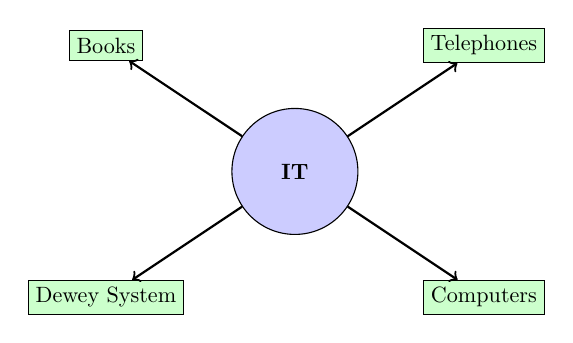
\begin{tikzpicture}[scale=0.8, every node/.style={transform shape}]
    % Central node
    \node[circle, draw, fill=blue!20, minimum size=2cm] (center) at (0,0) {\textbf{IT}};
    
    % Surrounding examples - mix of old and new
    \node[rectangle, draw, fill=green!20] (book) at (-3,2) {Books};
    \node[rectangle, draw, fill=green!20] (phone) at (3,2) {Telephones};
    \node[rectangle, draw, fill=green!20] (dewey) at (-3,-2) {Dewey System};
    \node[rectangle, draw, fill=green!20] (computer) at (3,-2) {Computers};
    
    % Arrows
    \draw[->, thick] (center) -- (book);
    \draw[->, thick] (center) -- (phone);
    \draw[->, thick] (center) -- (dewey);
    \draw[->, thick] (center) -- (computer);
\end{tikzpicture}
\end{center}

\end{frame}

% Slide 3: Why Ethics Matter
\begin{frame}{Why Ethics Matter in the Digital Age}

\begin{itemize}
    \item Information technologies have moved from being optional tools to essential infrastructure that shapes how we work, communicate, and understand the world.
    \item The rapid pace of technological change often outstrips our ability to develop appropriate ethical guidelines and legal frameworks to govern these technologies.
    \item Digital information is fundamentally different from physical resources because it can be copied infinitely without loss, raising unique questions about ownership and distribution.
    \item The choices we make about designing, deploying, and using information technologies will profoundly affect human flourishing for generations to come.
\end{itemize}

\begin{alertblock}{The Central Question}
Who should have the power to collect, control, and use the massive amounts of data generated by modern information technologies—and what moral principles should guide these decisions?
\end{alertblock}

\end{frame}

% Slide 4: What Is Information? (CORRECTED)
\begin{frame}{What Is Information? From Strings on Fingers to Smartphones}

\begin{itemize}
    \item \textbf{Information} can be understood as any useful data, instructions, or meaningful message content that helps shape our thoughts and actions.
    \item The word "information" literally means to "give form to" or to shape one's understanding of the world.
    \item A simple example: tying a string around your finger serves as information technology—the string symbolizes a complex proposition like "buy groceries before you come home."
    \item The string itself is not the information; it merely represents or symbolizes the information, which means it must be correctly interpreted to be useful.
\end{itemize}

\begin{center}
\begin{tabular}{lll}
\toprule
\textbf{Technology} & \textbf{Symbol/Medium} & \textbf{Information Represented} \\
\midrule
String on finger & Physical knot & "Remember to buy groceries" \\
Written letter & Ink on paper & Personal message to recipient \\
Book & Printed text & Knowledge or story \\
Smartphone alarm & Digital signal & "Wake up at 7:00am" \\
\bottomrule
\end{tabular}
\end{center}

\end{frame}

% Slide 5: Syntactical vs. Semantic Information
\begin{frame}{Syntactical vs. Semantic Information: Understanding the Difference (Shannon)}

\begin{itemize}
    \item \textbf{Syntax} refers to the structure and ordering of symbols in information, while \textbf{semantics} refers to the meaning or content that those symbols represent.
    \item Claude Shannon, working at Bell Labs in the 1940s, developed a mathematical theory of communication that focused on syntax—how to encode, transmit, and decode symbols while minimizing noise and errors.
    \item Shannon's approach treats \textbf{information} as \textit{meaningfully ordered sets of symbols that can be transmitted as signals}, but it deliberately leaves out questions about what those symbols actually mean.
\end{itemize}

\begin{block}{Why This Matters}
Modern computers are extraordinarily good at processing syntactical information (manipulating symbols according to rules), but whether they can truly understand the semantic meaning of that information remains a fundamental philosophical question.
\end{block}

\end{frame}

% Slide 6: The Chinese Room Argument
\begin{frame}{The Chinese Room Argument: Can Computers Really Think? (Searle)}

\begin{itemize}
    \item Philosopher John Searle (1980) proposed a thought experiment to argue that computers cannot truly understand information, even if they appear to process it intelligently.
    \item Imagine a person who doesn't speak Chinese locked in a room with a rulebook for manipulating Chinese characters—they receive Chinese stories and questions, then follow rules to output appropriate Chinese answers.
    \item The person in the room would produce correct answers without understanding anything about the stories, knowing only how to manipulate symbols according to syntactical rules.
    \item Searle argues that computers work the same way: they skillfully manipulate syntax without any genuine understanding of semantics or meaning.
\end{itemize}

\begin{center}
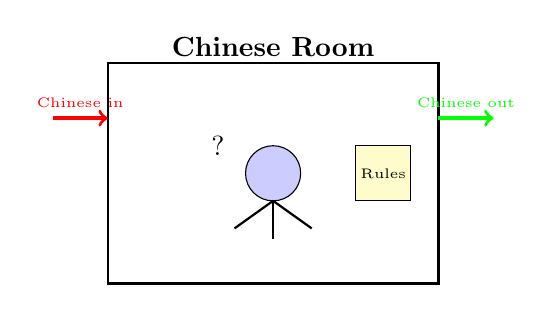
\begin{tikzpicture}[scale=0.7]
    % Room
    \draw[thick] (0,0) rectangle (6,4);
    \node at (3,4.3) {\textbf{Chinese Room}};
    
    % Person
    \draw[fill=blue!20] (3,2) circle (0.5);
    \draw[thick] (3,1.5) -- (3,0.8);
    \draw[thick] (3,1.5) -- (2.3,1);
    \draw[thick] (3,1.5) -- (3.7,1);
    
    % Rulebook
    \draw[fill=yellow!20] (4.5,1.5) rectangle (5.5,2.5);
    \node at (5,2) {\tiny Rules};
    
    % Input/Output
    \draw[->, very thick, red] (-1,3) -- (0,3) node[midway, above] {\tiny Chinese in};
    \draw[->, very thick, green] (6,3) -- (7,3) node[midway, above] {\tiny Chinese out};
    
    % Question mark over person
    \node at (2,2.5) {?};
\end{tikzpicture}
\end{center}

\end{frame}

% Slide 7: Three Functions of Information Technology
\begin{frame}{Three Functions of Information Technology: Record, Communicate, Organize}

\begin{itemize}
    \item All information technologies can be categorized by their function(s): \textbf{recording} (storing), \textbf{communicating} (transmitting), or \textbf{organizing/synthesizing} information.
    \item Many technologies perform multiple functions—for example, a smartphone can record photos, communicate via text messages, and organize your calendar appointments.
    \item The computer is unique as a \textbf{universal machine}: it can be programmed to emulate any form of information technology and perform all three functions simultaneously.
    \item Understanding these three functions helps us recognize the different ethical challenges that arise from each type of information processing.
\end{itemize}


\begin{center}
\begin{tabular}{lll}
\toprule
\textbf{Function} & \textbf{Classic Example} & \textbf{Digital Example} \\
\midrule
\textbf{Record} & Book, photograph & Cloud storage, database \\
\textbf{Communicate} & Telephone, letter & Email, text message \\
\textbf{Organize} & Dewey Decimal System & Search engine, algorithm \\
\bottomrule
\end{tabular}
\end{center}


\end{frame}

% NEW SLIDE 4: Information Technology in This Lecture (Insert after slide 3)
\begin{frame}{The Information Technologies Behind This Lecture}

\begin{itemize}
    \item This lecture itself demonstrates the layered nature of information technology—each layer building on previous innovations to enable new forms of communication and learning.
    \item \textbf{Written language} (ancient technology) allows us to record and transmit ideas across time; \textbf{mathematical notation} enables precise symbolic expression.
    \item \textbf{Von Neumann computer architecture} (1945) provides the computational foundation; \textbf{ASCII} (1963) standardizes character encoding for digital text.
    \item \textbf{LaTeX} (1980s) typesets these slides with mathematical precision; \textbf{VSCode with GitHub Copilot} (2021) provides AI-assisted coding; \textbf{GitHub} stores and versions the files; \textbf{Zoom} transmits the lecture; \textbf{YouTube} archives it for future viewing.
\end{itemize}

\begin{center}
    \scriptsize
\begin{tabular}{lll}
\toprule
\textbf{Technology} & \textbf{Year} & \textbf{Function} \\
\midrule
Written language & $\sim$3200 BCE & Record information \\
Von Neumann architecture & 1945 & Compute and process \\
ASCII & 1963 & Encode characters digitally \\
LaTeX & 1984 & Organize and present \\
GitHub & 2008 & Store and collaborate \\
Zoom/YouTube & 2011/2005 & Communicate and archive \\
Copilot and LLMs & 2021 & AI-assisted ``generative'' creation of LaTeX code \\
\bottomrule
\end{tabular}
\end{center}

\end{frame}

% Slide 8: What Is Ethics?
\begin{frame}{What Is Ethics? Understanding Moral Philosophy}

\begin{itemize}
    \item \textbf{Ethics} (or moral philosophy) is the systematic study of right and wrong, good and bad, and what we ought to do in various situations.
    \item Ethics asks fundamental questions: What makes an action right or wrong? What kind of person should I strive to be? How should we organize society fairly?
    \item Ethical thinking differs from simply following laws, customs, or personal preferences—it requires reasoned justification and consideration of principles that apply broadly.
    \item In this course, we'll use ethical frameworks to analyze the moral dimensions of information technologies and develop reasoned positions on controversial issues.
\end{itemize}

\begin{block}{Ethics vs. Other Forms of Guidance}
\begin{itemize}
    \item \textbf{Law}: What we are legally required or prohibited from doing
    \item \textbf{Custom/Etiquette}: What social conventions expect us to do
    \item \textbf{Religion}: What religious authorities or texts command
    \item \textbf{Ethics}: What we ought to do based on moral reasoning and principles
\end{itemize}
\end{block}

\end{frame}

% Slide 9: Normative vs Descriptive Ethics (REVISED)
\begin{frame}{Normative Ethics vs Descriptive Ethics}

\begin{itemize}
    \item \textbf{Descriptive ethics} studies how people actually behave and what moral beliefs they hold, without making judgments about whether those beliefs or behaviors are right or wrong.
    \item \textbf{Normative ethics} prescribes how people ought to behave and which moral principles should guide our actions, providing standards for evaluating conduct.
    \item In this course, we focus primarily on normative ethics—developing reasoned arguments about how information technologies should be designed and used, not merely describing current practices.
\end{itemize}

\begin{center}
    \scriptsize
\begin{tabular}{p{5cm}p{5cm}}
\toprule
\textbf{Descriptive Ethics} & \textbf{Normative Ethics} \\
\midrule
"Most people share their location data with apps." & "Should people share their location data with apps?" \\
\midrule
"62\% of teens say social media has no effect on their self-esteem." & "What responsibilities do social media companies have to protect teen wellbeing?" \\
\midrule
"Companies routinely collect browsing history." & "Is it morally permissible for companies to collect browsing history without explicit consent?" \\
\bottomrule
\end{tabular}
\end{center}

\end{frame}

% Slide 10: From Common Morality to Professional Ethics (REVISED AGAIN)
\begin{frame}{From Common Morality to Professional Ethics}

\begin{itemize}
    \item \textbf{Common morality} consists of basic moral norms shared across cultures—prohibitions against harm, theft, and deception, and requirements to help others and keep promises.
    \item However, information technologies create \textbf{novel moral problems} that common morality alone cannot resolve—issues our ancestors never faced and traditional moral wisdom doesn't directly address.
    \item \textbf{Applied ethics} and \textbf{professional ethics} extend common morality by developing specialized principles and reasoning for new contexts like healthcare, business, and information technology.
\end{itemize}

\begin{alertblock}{Why "Fourth Grade Morality" Isn't Enough}
Common morality tells us not to harm others and to respect their property—but it doesn't tell us whether collecting browsing data violates privacy, how to distribute algorithmic benefits justly, or who's responsible when an AI system causes harm. We need specialized ethical frameworks to extend basic moral principles to these novel technological situations.
\end{alertblock}

\end{frame}

% Slide 11: The Principalist Framework (REVISED)
\begin{frame}{The Principalist Framework: Five Key Principles}

\begin{itemize}
    \scriptsize
    \item The \textbf{principalist framework}, developed by Beauchamp and Childress for biomedical ethics and extended by Floridi for information ethics, provides five core principles for ethical analysis.
    \item The five principles are: \textbf{autonomy} (self-determination), \textbf{beneficence} (doing good), \textbf{non-maleficence} (avoiding harm), \textbf{justice} (fairness), and \textbf{explicability} (transparency and accountability).
    \item When principles conflict, we must use careful moral reasoning to determine which principle should take priority in a specific context.
\end{itemize}

\begin{center}
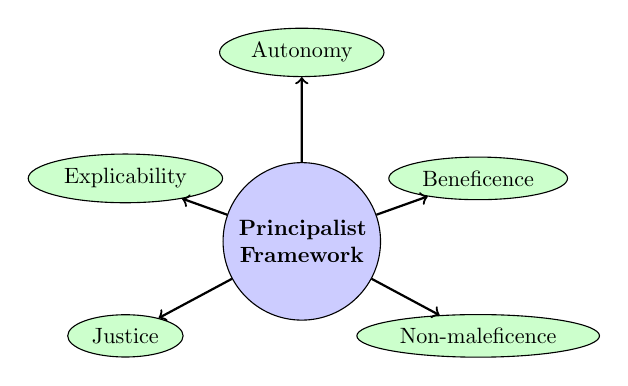
\begin{tikzpicture}[scale=0.8, every node/.style={transform shape}]
    % Central circle
    \node[circle, draw, fill=blue!20, minimum size=2.5cm, text width=2cm, align=center] (center) at (0,0) {\textbf{Principalist Framework}};
    
    % Five principles around it
    \node[ellipse, draw, fill=green!20] (auto) at (0,3) {Autonomy};
    \node[ellipse, draw, fill=green!20] (benef) at (2.8,1) {Beneficence};
    \node[ellipse, draw, fill=green!20] (nonmal) at (2.8,-1.5) {Non-maleficence};
    \node[ellipse, draw, fill=green!20] (just) at (-2.8,-1.5) {Justice};
    \node[ellipse, draw, fill=green!20] (explic) at (-2.8,1) {Explicability};
    
    % Arrows
    \draw[->, thick] (center) -- (auto);
    \draw[->, thick] (center) -- (benef);
    \draw[->, thick] (center) -- (nonmal);
    \draw[->, thick] (center) -- (just);
    \draw[->, thick] (center) -- (explic);
\end{tikzpicture}
\end{center}

\end{frame}

% Slide 12: Principle 1 - Autonomy (REVISED)
\begin{frame}{Principle of Autonomy: Respecting Self-Determination}

\begin{itemize}
    \item \textbf{Autonomy} is the capacity for self-determination—the ability to make informed decisions about one's own life based on one's values, preferences, and reasoning.
    \item Respecting autonomy means treating people as ends in themselves, not merely as means to others' goals, and ensuring they have meaningful control over decisions that affect them.
    \item In information technology contexts, autonomy requires informed consent for data collection, genuine choices about technology use, and freedom from manipulation or coercion.
\end{itemize}

\begin{alertblock}{Autonomy in IT: Key Questions}
\begin{itemize}
    \item Do users understand what data is being collected and how it will be used?
    \item Can users meaningfully choose whether to use a technology or share their data?
    \item Are users being manipulated through algorithmic recommendation systems?
    \item Do people have genuine control over their digital identities and information?
\end{itemize}
\end{alertblock}

\end{frame}

% Slide 13: Principle 2 - Beneficence
\begin{frame}{Principle of Beneficence: Promoting Good and Wellbeing}

\begin{itemize}
    \item \textbf{Beneficence} is the positive obligation to promote good, contribute to welfare, and help others flourish—going beyond merely avoiding harm.
    \item In information technology, beneficence requires designing systems that genuinely improve human lives, enhance capabilities, and contribute to individual and social wellbeing.
    \item This principle challenges us to ask whether technologies serve human needs or merely generate profit, and whether they empower or diminish human agency and connection.
\end{itemize}

\begin{block}{Beneficence in IT: Examples}
\textbf{Positive:} Health tracking apps that help people manage chronic conditions; educational platforms that increase access to learning; assistive technologies that enable people with disabilities.

\textbf{Questions to ask:} Does this technology make people's lives genuinely better? Does it enhance human capabilities or create new dependencies? Who benefits most from this technology?
\end{block}

\end{frame}

% Slide 14: Principle 3 - Non-maleficence
\begin{frame}{Principle of Non-maleficence: Above All, Do No Harm}

\begin{itemize}
    \item \textbf{Non-maleficence} embodies the ancient medical principle "first, do no harm"—we have an obligation to avoid causing harm to others through our actions.
    \item This principle requires us to anticipate potential harms from information technologies, including privacy violations, security breaches, psychological damage, and social harms.
    \item In IT contexts, harm can be direct (a data breach exposing personal information) or indirect (algorithms that perpetuate discrimination or social media features that contribute to mental health problems).
\end{itemize}

\begin{alertblock}{The Challenge of Unforeseen Harms}
Many information technologies cause harms that designers never anticipated—social media addiction, algorithmic bias in hiring, or cyberbullying platforms. Non-maleficence requires taking reasonable steps to identify and prevent potential harms before deployment.
\end{alertblock}

\end{frame}

% Slide 15: Principle 4 - Justice
\begin{frame}{Principle of Justice: Fairness and Equitable Distribution}

\begin{itemize}
    \item \textbf{Justice} requires fair distribution of benefits and burdens, equal treatment of equals, and special concern for vulnerable or disadvantaged groups.
    \item In information technology, justice addresses the digital divide, algorithmic bias, and whether technologies reinforce or reduce existing social inequalities.
    \item Justice questions include: Who has access to beneficial technologies? Whose interests do algorithms serve? Who bears the risks and costs of technological development?
\end{itemize}

\begin{center}
\begin{tabular}{ll}
\toprule
\textbf{Justice Concern} & \textbf{IT Example} \\
\midrule
Access inequality & Broadband access gaps \\
Algorithmic bias & Facial recognition errors for minorities \\
Exploitation & Data harvesting from vulnerable users \\
Fair treatment & Discriminatory hiring algorithms \\
\bottomrule
\end{tabular}
\end{center}

\end{frame}

% Slide 16: Principle 5 - Explicability
\begin{frame}{Principle of Explicability: Transparency and Accountability}

\begin{itemize}
    \item \textbf{Explicability}, added by philosopher Luciano Floridi, requires that information systems be transparent, understandable, and that those who design and deploy them be accountable for their effects.
    \item This principle demands that we can explain how systems work, justify their design choices, and hold someone responsible when things go wrong.
    \item Explicability is especially challenging with complex AI systems and algorithms that even their creators may not fully understand—the "black box" problem.
\end{itemize}

\begin{block}{Why Explicability Matters}
Without explicability, we cannot meaningfully exercise autonomy (we can't consent to what we don't understand), assess beneficence and non-maleficence (we can't evaluate unknown harms), or ensure justice (we can't detect hidden biases). Explicability enables all other principles.
\end{block}

\end{frame}

% Slide 16.5: Transition to Recording Information Issues
\begin{frame}{Applying Principles to Information Recording}

\begin{itemize}
    \item We've established our ethical framework—now we apply it to specific challenges posed by information technologies.
    \item The first major function of IT is \textbf{recording} (storing) information—creating databases, files, and digital records of human activities.
    \item Recording information raises novel ethical problems that common morality doesn't directly address: What counts as consent for data collection? Who owns recorded information about you? When is surveillance justified?
    \item We'll analyze these issues using our principalist framework—asking how recording technologies affect autonomy, beneficence, non-maleficence, justice, and explicability.
\end{itemize}

\begin{block}{The Ethical Stakes}
Modern recording technologies can capture and store virtually unlimited information about every person—creating unprecedented power imbalances between those who control data and those who generate it. This section explores how to navigate these novel moral challenges.
\end{block}

\end{frame}

% Slide 17: Digital Footprints (REVISED)
\begin{frame}{Digital Footprints: What Data Do You Leave Behind?}

\begin{columns}[T]
\begin{column}{0.58\textwidth}
\begin{itemize}
    \item Every digital action leaves a \textbf{data trail}—GPS coordinates, browser histories, purchases, and social media interactions.
    \item Modern technologies automatically collect biometric data, financial transactions, and search queries—creating comprehensive digital profiles.
    \item This collection often happens \textbf{behind the scenes} without users' awareness or meaningful consent.
\end{itemize}

\vspace{0.5cm}

\begin{alertblock}{Key Issue}
Aggregating seemingly innocent data points can reveal intimate details you never explicitly shared.
\end{alertblock}
\end{column}

\begin{column}{0.38\textwidth}
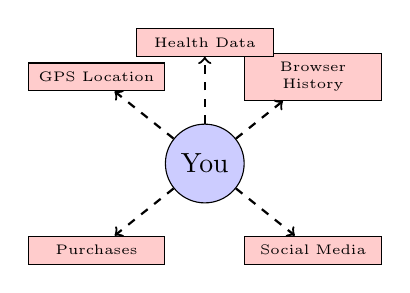
\begin{tikzpicture}[scale=0.55]
    % Central figure
    \node[circle, draw, fill=blue!20, minimum size=1cm] (person) at (0,0) {You};
    
    % Data trails
    \node[rectangle, draw, fill=red!20, text width=1.5cm, align=center, font=\tiny] (gps) at (-2.5,2) {GPS Location};
    \node[rectangle, draw, fill=red!20, text width=1.5cm, align=center, font=\tiny] (browse) at (2.5,2) {Browser History};
    \node[rectangle, draw, fill=red!20, text width=1.5cm, align=center, font=\tiny] (purchase) at (-2.5,-2) {Purchases};
    \node[rectangle, draw, fill=red!20, text width=1.5cm, align=center, font=\tiny] (social) at (2.5,-2) {Social Media};
    \node[rectangle, draw, fill=red!20, text width=1.5cm, align=center, font=\tiny] (health) at (0,2.8) {Health Data};
    
    % Arrows
    \draw[->, thick, dashed] (person) -- (gps);
    \draw[->, thick, dashed] (person) -- (browse);
    \draw[->, thick, dashed] (person) -- (purchase);
    \draw[->, thick, dashed] (person) -- (social);
    \draw[->, thick, dashed] (person) -- (health);
\end{tikzpicture}
\end{column}
\end{columns}

\end{frame}

% Slide 18: Privacy in the Digital Age (REVISED)
\begin{frame}{Privacy in the Digital Age: Who Owns Your Information?}

\begin{itemize}
    \item \textbf{Privacy} traditionally meant the ability to control access to one's personal space and information, but information technology has fundamentally challenged this concept.
    \item Philosopher Helen Nissenbaum argues that where physical barriers once protected privacy, technology now makes personal information "available at the click of a button or for a few dollars."
    \item The central ethical question is: who has the right to control, sell, or use information about you—especially when third parties collect it without your explicit knowledge or meaningful consent?
\end{itemize}

\begin{block}{The Death of Privacy?}
In 1999, Sun Microsystems CEO Scott McNealy famously declared: "You have zero privacy anyway. Get over it." While privacy may be harder to protect today, many philosophers argue that \textbf{personal autonomy and intimacy} still require us to defend privacy rights—even in the digital age. Without privacy protection, our autonomy is undermined.
\end{block}

\end{frame}

% Slide 19: The Cloud (REVISED)
\begin{frame}{The Cloud: Convenience vs. Control}

\begin{itemize}
    \item \textbf{Cloud storage} means your data is stored on remote servers owned by third parties (like Google, Apple, or Microsoft) rather than on devices you control.
    \item The cloud offers enormous convenience—access from anywhere, automatic backups, seamless syncing—but creates new vulnerabilities and trust dependencies.
    \item You're placing tremendous \textbf{trust} in third parties to protect your information, maintain access, and not misuse your data.
\end{itemize}

\begin{center}
\begin{tabular}{p{5cm}p{5cm}}
\toprule
\textbf{Benefits} & \textbf{Risks} \\
\midrule
Access from any device & Loss of direct control \\
Automatic backups & Company could lose/delete data \\
No local storage needed & Privacy breaches possible \\
Easy sharing with others & Uncertain legal protections \\
Professional security teams & Data mining by companies \\
\bottomrule
\end{tabular}
\end{center}

\end{frame}

% Slide 20: Biometric Data (REVISED)
\begin{frame}{Biometric Data: Your Body as Information}

\begin{itemize}
    \item \textbf{Biometric data} refers to measurements of your physical characteristics—fingerprints, facial recognition, heart rate, blood pressure, sleep patterns, and DNA sequences.
    \item Technologies like smartwatches and fitness trackers collect continuous biometric data streams, often shared with third-party applications and companies.
    \item Unlike passwords, you cannot change your fingerprints or facial structure—making biometric data breaches particularly serious and permanent violations.
\end{itemize}

\begin{alertblock}{Principalist Analysis}
\textbf{Autonomy}: Do users consent meaningfully? \textbf{Non-maleficence}: What harms result from breaches? \textbf{Justice}: Who has access to beneficial health tracking vs. whose data is exploited? \textbf{Explicability}: Can users understand how their biometric data is analyzed?
\end{alertblock}

\end{frame}

% Slide 21a: Case Study 1 - The Fitness Tracker Dilemma
\begin{frame}{Case Study 1: The Fitness Tracker Dilemma}

\begin{block}{The Scenario}
Ada, a high school senior, receives a fitness tracker as a gift. The device monitors her heart rate, sleep patterns, steps, and location throughout the day. The companion app offers personalized health insights and connects to a social network where users can share achievements and compete with friends.
\end{block}

\textbf{Key Facts:}
\begin{itemize}
    \item The privacy policy (12 pages of legal text) states that health data may be shared with "trusted third-party partners" for "service improvement."
    \item Ada's health insurance company offers a 15\% discount to customers who share fitness tracker data proving they exercise regularly.
    \item The app uses dark patterns—pre-checked boxes for data sharing and complex opt-out procedures buried in settings.
    \item Ada's school requires fitness trackers for PE class participation and shares aggregate student data with the district.
\end{itemize}

\end{frame}

% Slide 21b: Case Study 1 - Review Questions
\begin{frame}{Case Study 1: Review Questions}

\textbf{Using the Principalist Framework, analyze:}

\begin{enumerate}
    \item \textbf{Autonomy}: Does Ada have meaningful autonomy over her health data? Consider the length and complexity of the privacy policy, the school requirement, and the insurance incentive. What would genuine informed consent look like here?
    
    \item \textbf{Justice}: Is it fair that students must use fitness trackers for PE class? What about students who can't afford devices or have health conditions they wish to keep private? Does the insurance discount create unjust inequalities?
    
    \item \textbf{Non-maleficence}: What potential harms could result from sharing Ada's biometric and location data with third parties? Consider both immediate risks (data breaches) and long-term risks (discrimination, surveillance).

    \item \textbf{Explicability}: Who is accountable if Ada's data is misused? Can Ada meaningfully understand how her data will be analyzed and used by "trusted partners"?
\end{enumerate}

\end{frame}

% Slide 22: Privacy, Confidentiality, and Trust Online
\begin{frame}{Privacy, Confidentiality, and Trust Online}

\begin{columns}[T]
\begin{column}{0.60\textwidth}
\begin{itemize}
    \item Information technology forces us to rethink privacy concepts based on print technologies like letters and newspapers.
    \item \textbf{Confidentiality} refers to keeping specific information private between particular parties—like doctor-patient or lawyer-client communications.
    \item \textbf{Trust} becomes crucial when we must rely on third parties to protect our information and use it appropriately.
\end{itemize}

\begin{block}{Key Tension}
Digital information is easily shared and altered, stretching traditional privacy protections to their breaking point.
\end{block}
\end{column}

\begin{column}{0.38\textwidth}
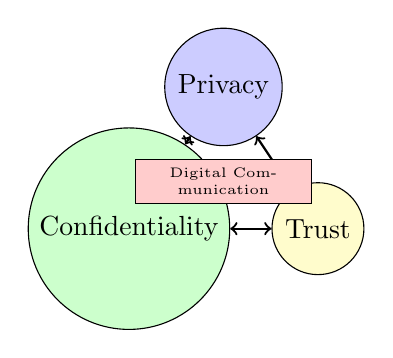
\begin{tikzpicture}[scale=0.6]
    % Triangle showing relationship
    \node[circle, draw, fill=blue!20] (priv) at (0,3) {Privacy};
    \node[circle, draw, fill=green!20] (conf) at (-2,0) {Confidentiality};
    \node[circle, draw, fill=yellow!20] (trust) at (2,0) {Trust};
    
    % Connecting lines
    \draw[<->, thick] (priv) -- (conf);
    \draw[<->, thick] (priv) -- (trust);
    \draw[<->, thick] (conf) -- (trust);
    
    % Central issue
    \node[rectangle, draw, fill=red!20, text width=2cm, align=center, font=\tiny] at (0,1) {Digital Communication};
\end{tikzpicture}

\vspace{0.3cm}

\textbf{Under pressure from:}
\begin{itemize}
    \item Easy copying
    \item Third-party access
    \item Data aggregation
    \item Unclear ownership
\end{itemize}
\end{column}
\end{columns}

\end{frame}

% Slide 23: Who Controls Your Personal Information?
\begin{frame}{Who Controls Your Personal Information?}

\begin{itemize}
    \item One fundamental question of information ethics: who has the final say over whether information about you is communicated, sold, or used?
    \item Philosopher Alan Westin argued that \textbf{control of access to personal information} is the key to privacy in the digital age—without control, privacy rights are meaningless.
    \item Traditional institutions (governments, banks, healthcare systems, corporations) have long held power through their control of stored information about individuals.
\end{itemize}

\begin{center}
\begin{tabular}{lll}
\toprule
\textbf{Your Data} & \textbf{Who Controls It?} & \textbf{Ethical Issue} \\
\midrule
Medical records & Hospital, insurance, govt & Privacy vs. public health \\
Financial history & Banks, credit agencies & Access vs. exploitation \\
Browsing history & ISPs, websites, advertisers & Tracking vs. consent \\
Email content & Email provider, govt & Confidentiality vs. security \\
Social media posts & Platform companies & Ownership vs. terms of service \\
\bottomrule
\end{tabular}
\end{center}

\end{frame}

% Slide 24: Digital Communication
\begin{frame}{Digital Communication: Email, Texts, and Social Media Ethics}

\begin{itemize}
    \item Digital communication technologies (email, text messages, social media) have transformed how we share information, but they create new ethical challenges regarding privacy, permanence, and context collapse.
    \item \textbf{Permanence}: Digital messages can be stored indefinitely, forwarded without permission, and retrieved years later—unlike ephemeral spoken conversations.
    \item \textbf{Context collapse}: Social media collapses multiple audiences (family, friends, employers, strangers) into one, making it nearly impossible to share appropriately for different contexts.
    \item The ease of copying and forwarding digital messages means confidential information can spread instantly beyond its intended recipients, violating trust and confidentiality norms.
\end{itemize}

\begin{alertblock}{Ethical Question}
If you send someone a private message, do they have the right to screenshot and share it? Does your expectation of privacy depend on the platform used? What obligations do we have regarding digital communications we receive?
\end{alertblock}

\end{frame}

% Slide 25: Contextual Integrity
\begin{frame}{Contextual Integrity: Privacy in Different Social Contexts}

\begin{columns}[T]
\begin{column}{0.50\textwidth}
\begin{itemize}
    \item Philosopher Helen Nissenbaum's theory of \textbf{contextual integrity} argues that privacy isn't about secrecy—it's about appropriate information flow for specific contexts.
    \item Information appropriate in one context (medical exam) becomes a privacy violation in another (dinner conversation).
    \item Social media and data aggregation violate contextual integrity by combining information from different contexts in unexpected ways.
\end{itemize}

\begin{block}{Key Insight}
Privacy violations occur when information flows in ways that violate context-specific norms, not just when secrets are revealed.
\end{block}
\end{column}

\begin{column}{0.38\textwidth}
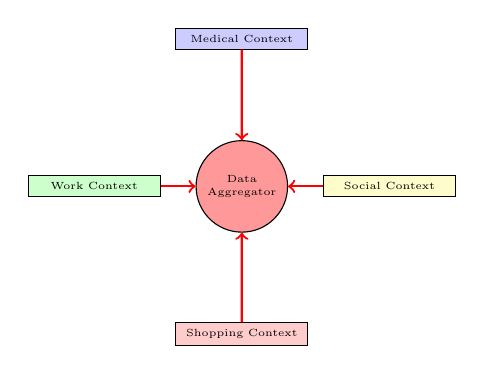
\begin{tikzpicture}[scale=0.75, every node/.style={transform shape}]
    % Different contexts
    \node[rectangle, draw, fill=blue!20, text width=2cm, align=center, font=\tiny] (med) at (0,3) {Medical Context};
    \node[rectangle, draw, fill=green!20, text width=2cm, align=center, font=\tiny] (work) at (-2.5,0.5) {Work Context};
    \node[rectangle, draw, fill=yellow!20, text width=2cm, align=center, font=\tiny] (social) at (2.5,0.5) {Social Context};
    \node[rectangle, draw, fill=red!20, text width=2cm, align=center, font=\tiny] (shop) at (0,-2) {Shopping Context};
    
    % Central violation
    \node[circle, draw, fill=red!40, minimum size=1.5cm, font=\tiny, text width=1.2cm, align=center] (data) at (0,0.5) {Data Aggregator};
    
    % Arrows showing inappropriate flow
    \draw[->, thick, red] (med) -- (data);
    \draw[->, thick, red] (work) -- (data);
    \draw[->, thick, red] (social) -- (data);
    \draw[->, thick, red] (shop) -- (data);
\end{tikzpicture}

\vspace{0.2cm}
\centering
\textit{\tiny Privacy violation through context collapse}
\end{column}
\end{columns}

\end{frame}

% Slide 26: Search Engines and Filter Bubbles
\begin{frame}{Search Engines and Filter Bubbles: How Algorithms Shape What You See}

\begin{itemize}
    \item \textbf{Search engines} organize the vast amount of information on the internet using algorithms that rank and filter results based on relevance, popularity, and personalization.
    \item \textbf{Filter bubbles} occur when algorithms selectively present information based on your past behavior, creating a personalized information environment that reinforces existing beliefs.
    \item These systems raise serious concerns about \textbf{autonomy}—can you make truly informed decisions if algorithms control what information reaches you?
    \item Questions of \textbf{justice} emerge when different users receive systematically different information based on their demographics, location, or wealth.
\end{itemize}

\begin{center}
\begin{tabular}{ll}
\toprule
\textbf{Algorithm Feature} & \textbf{Ethical Concern} \\
\midrule
Personalized results & Filter bubble effect \\
Ranking by popularity & Amplifies majority views \\
Ad-based revenue model & Prioritizes engagement over truth \\
Opaque decision-making & Violates explicability \\
\bottomrule
\end{tabular}
\end{center}

\end{frame}

% Slide 27: Data Mining and the Power of Information Control
\begin{frame}{Data Mining and the Power of Information Control}

\begin{itemize}
    \item \textbf{Data mining} refers to analyzing large datasets to discover patterns, correlations, and insights that weren't visible in smaller samples or individual cases.
    \item Companies and governments use data mining to predict behavior, target advertising, assess risk, and make decisions about individuals—often without those individuals' knowledge.
    \item The control of information represents a form of \textbf{political and economic power}—those who can collect, analyze, and act on data have significant advantages over those who cannot.
\end{itemize}

\begin{block}{The Power Asymmetry}
Organizations increasingly possess detailed profiles of billions of individuals, while those individuals often lack access to their own data or understanding of how it's used. This creates a fundamental \textbf{justice} problem: unequal power, unequal access, and unequal vulnerability to harm. As philosopher Richard Mason argued, these technologies require us to rethink the social contract itself.
\end{block}

\end{frame}

% Slide 28a: Case Study 2 - Bias in Google Search and ChatGPT
\begin{frame}{Case Study 2: Bias in Google Search and ChatGPT}

\begin{block}{The Scenario}
Marcus, a high school junior, is researching "successful CEOs" for a business class project. He uses Google Search and ChatGPT to find information and generate ideas.
\end{block}

\textbf{Key Facts:}
\begin{itemize}
    \item Google's image search for "successful CEO" returns predominantly images of white men in business suits, with very few women or people of color in the top 100 results.
    \item When Marcus asks ChatGPT to "describe a typical successful CEO," the AI generates a description matching traditional stereotypes: "confident," "assertive," "male," "experienced in finance."
    \item ChatGPT was trained on internet text data that reflects historical biases and underrepresentation of women and minorities in leadership positions.
    \item Neither Google nor ChatGPT explicitly explains how their algorithms work or why certain results appear first—the decision-making process is largely opaque.
    \item Marcus doesn't realize these results are algorithmically curated and might be biased—he treats them as objective information.
\end{itemize}

\end{frame}

% Slide 28b: Case Study 2 - Review Questions
\begin{frame}{Case Study 2: Review Questions}

\textbf{Using the Principalist Framework, analyze:}

\begin{enumerate}
    \item \textbf{Justice}: How do biased search results and AI outputs perpetuate existing inequalities? Who is harmed when algorithms reinforce stereotypes about leadership, success, or capability? What obligations do tech companies have to ensure fair representation?
    
    \item \textbf{Autonomy}: Can Marcus make truly autonomous decisions about his understanding of business leadership if algorithms control what information he sees? Does the lack of awareness about algorithmic curation undermine informed decision-making?
    
    \item \textbf{Explicability}: Should Google and OpenAI be required to explain how their algorithms rank results and generate text? Who is accountable when biased outputs cause harm? Can users meaningfully understand these systems?
    
    \item \textbf{Beneficence/Non-maleficence}: What are the broader social harms of algorithmic bias in information systems? How might this affect career aspirations, hiring decisions, and social perceptions?
\end{enumerate}

\end{frame}

% Slide 29: Social Media Ethics
\begin{frame}{Social Media Ethics: Friendship, Identity, and Authenticity}

\begin{itemize}
    \item Social media platforms fundamentally reshape how we form and maintain relationships, raising questions about the nature of \textbf{friendship}, \textbf{identity}, and \textbf{authenticity} in digital spaces.
    \item Philosopher Shannon Vallor argues that social media can support genuine friendships and human flourishing—or it can cultivate vice and shallow connections, depending on how platforms are designed and used.
    \item The architecture of social media (likes, followers, metrics) can encourage performative behavior and superficial engagement rather than deep, meaningful relationships.
    \item \textbf{Virtue ethics} asks: what kind of character traits do social media platforms cultivate? Do they encourage honesty, compassion, and wisdom—or vanity, envy, and distraction?
\end{itemize}

\begin{alertblock}{The Authenticity Problem}
Social media allows us to curate idealized versions of ourselves, but this can create pressure to maintain false personas and prevent genuine self-disclosure. How can we cultivate authentic relationships when the medium encourages performance over authenticity?
\end{alertblock}

\end{frame}

% Slide 30: Online Gaming Communities (REVISED)
\begin{frame}{Online Gaming Communities: Real Ethics in Virtual Worlds}

\begin{itemize}
    \item \textbf{Massively multiplayer online games} (MMOs) create virtual worlds where millions of people interact, form communities, and develop alternative lives.
    \item These virtual worlds raise real ethical questions: Do our moral obligations extend to virtual spaces? Can you wrong someone in a game?
    \item Players develop genuine relationships, economies, and social structures within games—suggesting that virtual interactions have real moral significance.
    \item Griefing, harassment, and discrimination in games cause real psychological harm to real people, even if the environment is virtual.
\end{itemize}

\begin{exampleblock}{Real-World Case: RuneScape Theft (2007)}
In the Netherlands, two teenagers physically assaulted a 13-year-old boy, beating and threatening him with a knife until he logged into the game RuneScape and transferred his virtual amulet and mask to them. In 2012, the Dutch Supreme Court upheld their theft conviction, ruling that virtual objects have "intrinsic value" because of "the time and energy invested" in obtaining them. The offenders received 144 hours of community service.
\end{exampleblock}

\end{frame}

% Slide 31: Digital Identities
\begin{frame}{Digital Identities: Who Are You Online?}

\begin{itemize}
    \item Our \textbf{digital identities}—the personas we create and maintain online—raise profound questions about authenticity, consistency, and self-presentation across different platforms and contexts.
    \item Social media encourages us to curate idealized versions of ourselves, potentially creating a gap between our online persona and our actual lived experience.
    \item Multiple digital identities (professional LinkedIn, casual Instagram, anonymous Reddit) fragment the self, raising questions about which version is "really you."
    \item The permanence of digital identities creates new challenges—online posts from years ago can resurface and affect current opportunities, relationships, and reputation.
\end{itemize}

\begin{block}{The Authenticity Question}
Philosopher Shannon Vallor argues we must ask: Do our online identities reflect genuine self-expression and help us flourish as human beings? Or do they trap us in performative cycles that prevent authentic connection and self-knowledge? The architectures of social media platforms shape which aspects of ourselves we present—and therefore who we become.
\end{block}

\end{frame}

% Slide 32: The Technological Transparency Paradox (REVISED)
\begin{frame}{The Technological Transparency Paradox: Freedom vs. Control}

\begin{itemize}
    \item Digital information creates a fundamental paradox: "Information wants to be free" (easily copied and shared) versus "Information is valuable and should be controlled" (property requiring protection).
    \item Unlike physical objects, digital information is \textbf{nonexclusory}—we can all possess the same digital file without preventing others from having it, since copying doesn't eliminate the original.
    \item This creates moral tensions: Should digital music, books, and movies be freely shared? Do creators have rights to control copies? Is piracy theft or liberation?
    \item The paradox extends to personal data: we want our information protected (privacy) but also want free access to others' information (transparency).
\end{itemize}

\begin{block}{The CIA Triad in Tension}
    \scriptsize
Information security balances three goals:
\begin{itemize}
    \item \textbf{Confidentiality}: Keeping information private and controlled
    \item \textbf{Integrity}: Ensuring information remains accurate and unaltered
    \item \textbf{Availability}: Making information accessible when needed
\end{itemize}
These goals often conflict—maximizing availability threatens confidentiality; strict confidentiality limits availability. Finding the right balance requires careful ethical reasoning.
\end{block}

\end{frame}
% Slide 33: Malware and Cybersecurity
\begin{frame}{Malware and Cybersecurity: Protecting Digital Systems}

\begin{itemize}
    \item \textbf{Malware} (malicious software) includes viruses, worms, trojans, ransomware, and spyware designed to damage systems, steal data, or enable unauthorized access.
    \item \textbf{Cybersecurity} involves protecting information systems from malware and unauthorized access, but it raises ethical tensions between security and privacy, convenience and protection.
    \item The ethics of cybersecurity involves questions of \textbf{non-maleficence} (preventing harm from attacks) and \textbf{justice} (who bears the costs and risks of security measures).
\end{itemize}

\begin{center}
\begin{tabular}{lll}
\toprule
\textbf{Malware Type} & \textbf{Function} & \textbf{Primary Harm} \\
\midrule
Virus & Replicates and spreads & System damage, data loss \\
Ransomware & Encrypts files for ransom & Extortion, business disruption \\
Spyware & Monitors user activity & Privacy violation \\
Trojan & Disguised malicious code & Unauthorized access \\
\bottomrule
\end{tabular}
\end{center}

\end{frame}

% Slide 34: Cyberwarfare and the Ethics of Digital Weapons
\begin{frame}{Cyberwarfare and the Ethics of Digital Weapons}

\begin{itemize}
    \item \textbf{Cyberwarfare} refers to using information technologies as weapons to attack enemy information systems, infrastructure, and military capabilities.
    \item These attacks can disable power grids, disrupt communications, destroy data, and potentially cause physical harm—all without traditional kinetic weapons.
    \item Cyberweapons raise novel ethical questions: Can they distinguish between military and civilian targets? Who is responsible for collateral damage? Do traditional rules of warfare apply?
\end{itemize}

\begin{block}{The Stuxnet Case}
Stuxnet (discovered 2010) was a sophisticated computer worm that targeted Iranian nuclear facilities, damaging centrifuges and setting back their nuclear program. Some argue it prevented military action that would have caused greater civilian casualties. Others worry it opened the door to continuous low-level cyber conflicts that avoid accountability and escalate slowly. The attack raised questions about \textbf{proportionality}, \textbf{discrimination}, and whether cyber operations can ever satisfy just war principles.
\end{block}

\end{frame}


% Slide 35: Artificial Intelligence
\begin{frame}{Artificial Intelligence: Can Machines Make Moral Decisions?}

\begin{itemize}
    \item \textbf{Artificial Intelligence (AI)} refers to information technologies that exhibit aspects of human-level intelligence, problem-solving, and decision-making capabilities.
    \item Alan Turing proposed in 1950 that machines would eventually "think" in ways indistinguishable from humans—the famous \textbf{Turing Test} where a computer tries to convince a human it's not a machine.
    \item Modern AI systems (like ChatGPT, facial recognition, and recommendation algorithms) raise urgent ethical questions about bias, accountability, and whether machines can or should make moral judgments.
    \item Key debate: Does consciousness matter for moral agency? Some argue we can only have moral duties toward conscious beings; others argue AI systems can have moral rights and duties regardless of consciousness.
\end{itemize}

\begin{alertblock}{The Moral Machine Problem}
If AI systems make decisions affecting human welfare (medical diagnoses, loan approvals, criminal sentencing), who is morally responsible when they err? The programmer? The company? The AI itself? Can we program machines to behave ethically, or does morality require something machines cannot possess?
\end{alertblock}

\end{frame}

% Slide 36: Robotics in Society (REVISED)
\begin{frame}{Robotics in Society: From Healthcare to Warfare}

\begin{itemize}
    \item \textbf{Robotics} combines information technology with physical machines that interact directly with humans and the environment.
    \item Applications range from medical robots assisting surgery to military drones conducting warfare—each raising distinct ethical challenges.
    \item \textbf{Military robotics} is especially controversial: autonomous weapons can make life-or-death decisions with little human intervention.
    \item Some ethicists argue robots could reduce casualties by following international humanitarian law more consistently than humans under stress; others worry autonomous weapons make war too easy to declare and violate human dignity by removing human judgment from killing decisions.
\end{itemize}

\begin{block}{Principalist Analysis of Military Robotics}
\textbf{Autonomy}: Do civilians consent to being potential targets of autonomous systems? \textbf{Non-maleficence}: Can robots reliably distinguish combatants from civilians and avoid excessive harm? \textbf{Justice}: Who bears responsibility when autonomous weapons cause unjust casualties? \textbf{Explicability}: Can military robots explain their targeting decisions?
\end{block}

\end{frame}

% Slide 37: The Future of Humanity (REVISED)
\begin{frame}{The Future of Humanity: Technology and Human Enhancement}

\begin{itemize}
    \item \textbf{Transhumanism} is the view that we should use technology to enhance human capabilities—extending lifespan, augmenting intelligence, and transcending biological limitations.
    \item \textbf{Moore's Law} observed that computing power doubles approximately every 18 months—futurist Ray Kurzweil predicts this acceleration could lead to "the Singularity," where technology fundamentally transforms human nature.
    \item Critics argue transhumanism reflects pseudoscientific beliefs and fear of death, devalues the natural human body, and would deepen inequality between enhanced and unenhanced humans.
\end{itemize}

\begin{center}
\begin{tabular}{p{4.5cm}p{5.5cm}}
\toprule
\textbf{Enhancement Type} & \textbf{Ethical Concerns} \\
\midrule
Cognitive enhancement & Fairness in education/work, authenticity, coercion \\
Life extension & Justice in resource distribution, overpopulation \\
Physical augmentation & Access inequality, redefining human dignity \\
Brain-computer interfaces & Privacy of thoughts, personal identity, autonomy \\
\bottomrule
\end{tabular}
\end{center}

\end{frame}


% Slide 38a: Case Study 3 - Being Young in the Age of LLMs (REVISED)
\begin{frame}{Case Study 3: Being Young in the Age of LLMs}

\begin{block}{The Scenario}
Maria is a high school senior trying to prepare for her future in a world rapidly being transformed by large language models (LLMs) like ChatGPT. She's watching how AI is changing writing, creative work, coding, research, and even social interaction—and wondering what this means for her generation.
\end{block}

\textbf{Key Facts:}
\scriptsize
\begin{itemize}
    \item Maria used to love writing stories and essays, but now wonders if developing writing skills matters when AI can generate high-quality text instantly. She's uncertain which skills will be valuable in 10 years.
    \item Her older cousin, a junior copywriter, just lost his job because the marketing firm replaced their writing team with two "AI coordinators" who edit AI-generated content.
    \item Maria notices her younger brother (age 12) primarily interacts with AI chatbots for entertainment, homework help, and even emotional support—he seems to prefer AI conversations to human ones.
    \item She observes that AI systems reflect and amplify existing biases, spread misinformation convincingly, and that her generation will inherit both the benefits and harms of these systems they didn't create.
\end{itemize}

\end{frame}

% Slide 38b: Case Study 3 - Review Questions (REVISED)
\begin{frame}{Case Study 3: Review Questions}

\textbf{Using the Principalist Framework, analyze:}

\begin{enumerate}
    \item \textbf{Autonomy \& Human Flourishing}: How do LLMs affect young people's development of critical thinking, creativity, and authentic self-expression? Does relying on AI for writing, problem-solving, and social interaction undermine the autonomy that comes from developing these capacities yourself? What does it mean to flourish as a human in an AI-saturated world?
    
    \item \textbf{Justice}: Is it fair that Maria's generation must navigate a transformed job market they didn't create? Who benefits most from LLM technology—tech companies, certain workers, society broadly? How should we address employment displacement? Do young people have a voice in how these transformative technologies are developed and deployed?
    
    \item \textbf{Non-maleficence}: What are the potential harms to young people from widespread LLM use—loss of skills, social isolation, exposure to bias and misinformation, psychological dependence? Who is responsible for preventing or mitigating these harms?
    
    \item \textbf{Beneficence}: What positive obligations do we have to ensure LLMs benefit rather than harm the next generation? Should education change? Should there be age restrictions or protections?
\end{enumerate}

\end{frame}


% Slide 39: Programming Morality
\begin{frame}{Programming Morality: Can We Build Ethical Machines?}

\begin{itemize}
    \item As AI systems make increasingly consequential decisions, computer scientists and philosophers are attempting to program machines that can reason about moral questions and behave ethically.
    \item \textbf{Machine morality} faces fundamental challenges: How do we translate complex ethical principles into code? Whose values should machines embody? Can algorithms capture moral nuance and context?
    \item Some approaches include programming explicit rules (like Asimov's Three Laws of Robotics), training AI on human moral judgments, or designing systems that can learn and adapt their moral reasoning.
    \item The challenge isn't just technical—it's philosophical: we must first achieve clarity about human ethics before we can teach ethics to machines.
\end{itemize}

\begin{block}{Information Ethics as a Framework}
    \scriptsize
Philosopher Luciano Floridi argues that information technologies themselves are becoming moral agents in our world—not because they're conscious, but because they shape the \textbf{infosphere} (the information environment) in which we live. We must design technologies that promote human flourishing, protect autonomy, distribute benefits justly, avoid harm, and remain explicable and accountable. Information ethics extends our moral framework to encompass the unique challenges of our digital age.
\end{block}

\end{frame}

% Slide 40: Your Digital Future
\begin{frame}{Your Digital Future: Becoming Ethical Technology Citizens}

\begin{itemize}
    \item You are growing up in a world where information technologies are not optional tools but essential infrastructure shaping every aspect of human life.
    \item The decisions your generation makes about designing, deploying, regulating, and using these technologies will determine whether they enhance or diminish human flourishing for decades to come.
    \item \textbf{Ethical technology citizenship} requires: understanding how technologies work, recognizing their moral implications, demanding accountability and explicability, and participating in democratic decisions about technological futures.
\end{itemize}

\begin{alertblock}{Your Responsibility and Your Power}
Richard Mason argued in 1986 that information technologies require us to rethink the social contract itself. That task now falls to you. You have both the \textbf{responsibility} to think critically about the ethical dimensions of technology and the \textbf{power} to shape a digital future that respects autonomy, promotes beneficence, avoids harm, ensures justice, and maintains explicability. The common morality you inherited is necessary but not sufficient—you must extend it thoughtfully to meet challenges your ancestors never imagined.
\end{alertblock}

\end{frame}

\end{document}

\end{document}